% Please use the skeleton file you have received in the
% invitation-to-submit email, where your data are already
% filled in. Otherwise please make sure you insert your
% data according to the instructions in PoSauthmanual.pdf
\documentclass{PoS}
\usepackage{amsmath}
\usepackage{color}
\definecolor{David}{rgb}{0.0,1.0,0.0}
\newcommand{\dgr}[1]{\textcolor{David}{#1}}

\title{Matrix elements from moments of correlation functions}

\ShortTitle{Moments of correlation functions}

\author{\speaker{Chia Cheng Chang}\\
        Lawrence Berkeley National Laboratory\\
        E-mail: \email{chiachang@lbl.gov}}
        
\author{Chris Bouchard\\
                The College of William \& Mary\\
                E-mail: \email{cmbouchard@wm.edu}}
                
\author{Kostas Orginos\\
                The College of William \& Mary \\
Thomas Jefferson National Accelerator Facility\\
E-mail: \email{kostas@wm.edu}}

\author{David Richards\\
Thomas Jefferson National Accelerator Facility\\
E-mail: \email{djr@jlab.org}}

\abstract{Momentum-space derivatives of matrix elements can be related
  to their coordinate-space moments through the Fourier transform. We
  derive these expressions as a function of momentum transfer $Q^2$
  for asymptotic in/out states consisting of a single hadron.  We
  calculate corrections to the finite volume moments by studying the
  spatial dependence of the lattice correlation functions.  This
  method permits the computation of not only the values of matrix
  elements at momenta accessible on the lattice, but also the
  momentum-space derivatives, providing {\it a priori} information
  about the $Q^2$ dependence of form factors. As a specific
  application we use the method, at a single lattice spacing and with
  unphysically heavy quarks, to directly obtain the slope of the
  isovector form factor at various $Q^2$, whence the isovector charge
  radius. The method has potential application in the calculation of
  any hadronic matrix element with momentum transfer, including those
  relevant to hadronic weak decays.}

\FullConference{34th annual International Symposium on Lattice Field Theory\\
		24-30 July 2016\\
		University of Southampton, UK}


\begin{document}

\section{Introduction}
Direct calculations of the \dgr{momentum-dependent} slopes of hadronic form factors
%correlation functions
allows for model independent determinations of physical observables
such as the charge radius of the proton.  Current experimental tension
for the proton charge radius stands at a startling $7\sigma$ between
electron and muonic measurement~\cite{Carlson:2015jba}. A model
independent lattice QCD calculation of the charge radius at the 2\%
level is necessary to discriminate the 4\% difference between electron
and muon probes. \dgr{Similarly, there is a $2\sigma$ tension between
  the nucleon axial mass, parameterising the $Q^2$ dependence of
  the nucleon axial form factor $F_A(Q^2)$ under a dipole ansatz and related to the inverse of the axial radius, obtained from}
%Resolution of the nucleon axial mass, related to the inverse of
%  the axial radius, experiences a 2 standard deviation tension between
  quasi-elastic scattering and electroproduction
  experiments~\cite{Anikin:2016teg}.
  The nucleon axial mass is
  %used
  %to determine the shape of the axial form factor $F_A(q^2)$ for
%  non-zero momentum transfer under the dipole ansatz, and is the
  \dgr{ the leading uncertainty when interpreting neutrino scattering
    experiments in the quasi-elastic regime.}  \dgr{\bfseries I'm not
    sure I understand the next statement.  Should this be up to $Q^2 =
    100~{\rm MeV}^2$?} A direct lattice QCD calculation of $F_A(Q^2)$
  with momentum transfer up to $\sim100~\text{GeV}^2$, in conjunction
  with the corresponding slopes may be used together in a model
  independent $z$-expansion~\cite{Bhattacharya:2011ah} in order to
  constrain $F_A(Q^2)$.  A target uncertainty of 1\% for $F_A(0)$,
  unobtainable with current lattice techniques and
  computer resources~\cite{Bhattacharya:2016zcn}, is desired to interpret next
  generation neutrino experiments such as the Deep Underground
  Neutrino Experiment (DUNE);
\dgr{at higher levels of precision,} isospin and electromagnetic
  corrections dominate.  Similarily, in conjunction with precision
  flavor physics experiments, lattice QCD calculations of the shape of
  form factors for semi-leptonic decays such as $B_s\rightarrow K \ell
  \nu$~\cite{Bouchard:2014ypa}, is used to constrain Standard Model
  parameters such as $|V_{ub}|$. \dgr{\bfseries This should be B to pi?}  The dominant error at large momentum
  transfer comes from the uncertainty in the form factors. The
  additional information provided by explicit lattice calculations of
  the slope may be used to reduce the uncertainty of the form factors
  across all momenta.

Application of coordinate-space moment methods was first introduced in
the mid 90's as a way to access the slope of the Isgur-Wise function
$\xi(\omega)$ at zero-recoil, in order to enable experimental results
obtained near zero-recoil in $B\rightarrow D$ semi-leptonic decays
\dgr{to be used to provide a value for $\mid V_{cb}\mid$}~\cite{Lellouch:1994zu}. At the turn of the millenium,
moment methods were used to calculate the slope of the
energy-momentum-tensor form factor, which is directly related to the
the angular momentum contribution to the spin of the
nucleon~\cite{Mathur:1999uf}\cite{Gadiyak:2001fe}. Recently, there is
revitalized interest in coordinate-space moment methods both in
applications to hadronic vacuum polarization
calculations~\cite{Chakraborty:2016mwy}\cite{Blum:2016xpd} in particle
physics, and to direct calculations of the anomolous magnetic moment of
the nucleon and nucleon radii in nuclear
physics~\cite{Alexandrou:2016rbj}. In parallel, momentum-space
derivative methods are also being explored to access similar nucleon
structure calculations such as the anomolous magnetic moment and
various nucleon radii~\cite{deDivitiis:2012vs}\cite{Tiburzi:2014yra}.
In these proceedings, we present a coordinate-space method that
directly calculates the slope of single particle form factors with
respect to 3- and 4-momentum squared at any lattice accessible
momenta.

\section{Formalism}
Correlators constructed from coordinate-space moment methods
%are known to have
\dgr{can have} zero overlap with the \dgr{states at zero momentum, and in particular the zero-momentum ground state}
%ground state
, and an example shown in
Ref.~\cite{Wilcox:2002zt} was instead shown to have overlap starting with the
lowest non-zero lattice momentum mode. The subtlety lies in the fact
that in Ref.~\cite{Wilcox:2002zt}, an odd spatial moment (or more
specifically a linear moment) is taken in order to calculate the
anomolous magnetic moment. Naively, as one takes the projection to
zero momentum with an odd spatial moment, the correlator would vanish
due to the oddness of the spatial integral.  However, the cancellation
does not occur when an even spatial moment is constructed, and is in
fact \dgr{illustrated} in a second example given in
Ref.~\cite{Wilcox:2002zt}. We derive in the following sections the
moment correlator and fit ansatz, and show that for all values of
momenta, even spatial moments are constructed, yielding overlap with
the desired ground state.

\subsection{Moments of correlation functions}
\begin{figure}[h]
	\centering
		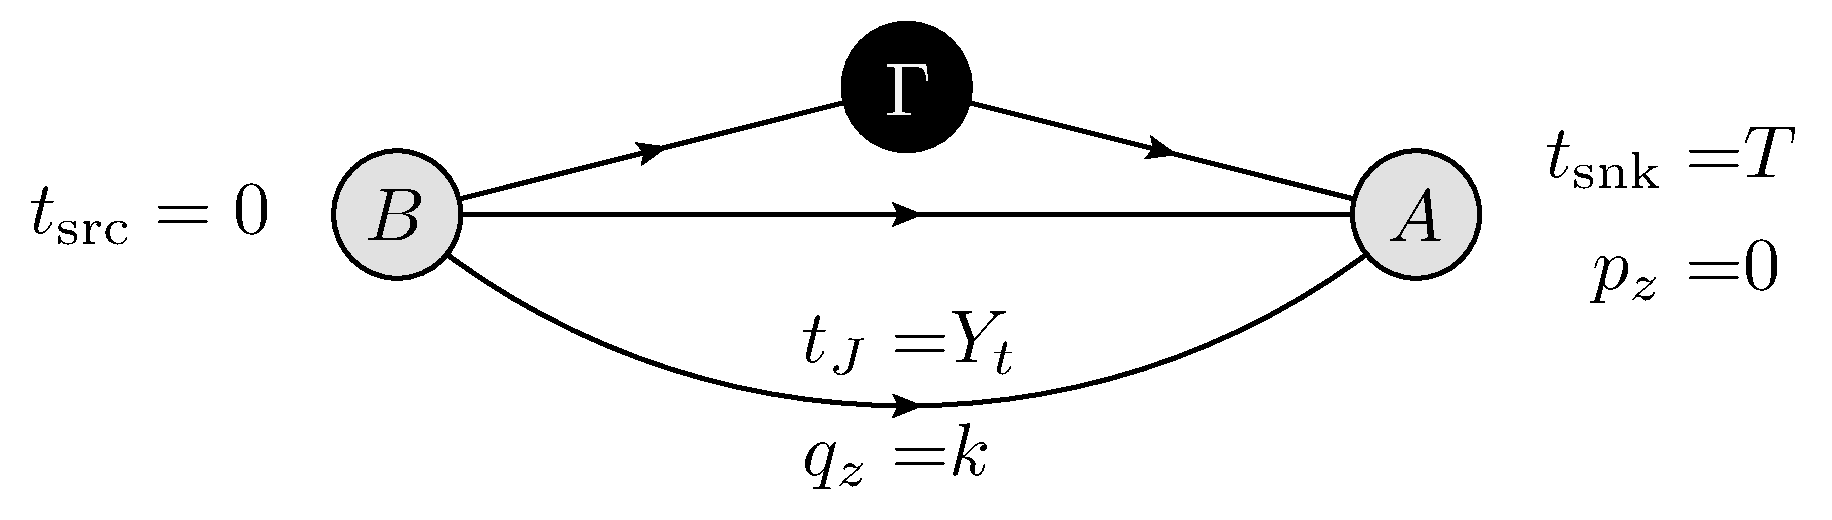
\includegraphics[width=0.75\textwidth]{./3pt_kinematics.pdf}
	\caption{Kinematics of the three-point correlator with baryon initial and final states. We work in the rest frame of the final hadron. The diagram for semi-leptonic decays \dgr{of mesons} involves only one spectator quark, but involves the same kinematics.}
	\label{fig:3pt_kinematics}
\end{figure}

Given a three-point correlation function with the initial state at
rest, and current insertion with three-momentum $k$ where, without loss of generality,  $k$ points
in the $z$-direction, as shown in
Fig.~\ref{fig:3pt_kinematics}, the three-momentum-projected
three-point correlation function has the general form,
\begin{align}
C^{\text{3pt}}(t_x, t_y;k) = \int d^3\vec{X} \int d^3\vec{Y} \left<A_{X_t,\vec{X}}|\Gamma_{Y_t,\vec{Y}} |B_{0,\vec{0}}\right> e^{-ikY_z},
\label{eq:3pt}
\end{align}
where translational invariance allows us to shift the sink to the
origin $\vec{x}^\prime = 0$ and the source to $\vec{X}\equiv \vec{x} -
\vec{x}^\prime$. \dgr{\bfseries I wonder if it is really necessary to
  mention translation invariance here, and just label things $X$ and
  $Y$ since this is such a common consruction, i.e. just use $\vec{x}, t_x,
  \vec{y}, t_y$, and also add $k$ as an argument to correlation function} \dgr{\bfseries Also, I wonder if the notation is
  perhaps a little confusing in terms of mixing up ``matrix elements''
  and ``correlation functions''.  We could write $\langle A_{X_t,
    \vec{X}} \Gamma_{Y_t, \vec{Y}} B_{0,\vec{0}}\rangle$ } Since the
source has zero three-momentum, the only momentum dependence left is
at the current insertion. The operators $A$ and $B$ are the source and
sink interpolation operators respectively, while $\Gamma$ is a generic
current insertion at position $\vec{Y}\equiv \vec{y}-\vec{x}^\prime$.

The derivative of the three-point correlator with respect to $k^2$ follows,
\begin{align}
C^\prime_{\text{3pt}}(t_x, t_y) = &\frac{\partial}{\partial k^2}C_{\text{3pt}}(t_x, t_y),\nonumber\\
=& \int d^3\vec{X} \int d^3\vec{Y} \left<A_{X_t,\vec{X}}|\Gamma_{Y_t,\vec{Y}} |B_{0,\vec{0}}\right> \left(\frac{-Y_z}{2k}\right)\sin\left(kY_z\right),
\label{eq:3ptmoment}
\end{align}
where in Eq.~(\ref{eq:3ptmoment}), the cosine component vanishes due
to symmetry. \dgr{\bfseries This next sentence may be a little
  pedantic for the lattice write-up}.  Commuting the $k^2$ derivative
across the integral, results in the derivative acting only on the
exponential, since the correlator is defined in spatial
coordinates. In the limit of zero momentum, the $k^2 \rightarrow 0$
limit of the integrand is given by L'H\^opital's rule,
\begin{align}
\lim_{k^2 \rightarrow 0} C^\prime_{\text{3pt}}(t_x, t_y) = & \int d^3\vec{X} \int d^3\vec{Y}\left(\frac{-Y_z^2}{2}\right)\left<A_{X_t,\vec{X}}|\Gamma_{Y_t,\vec{Y}} |B_{0,\vec{0}}\right>.
\label{eq:3ptmoment0}
\end{align}

%\begin{figure}[h]
%	\centering
%		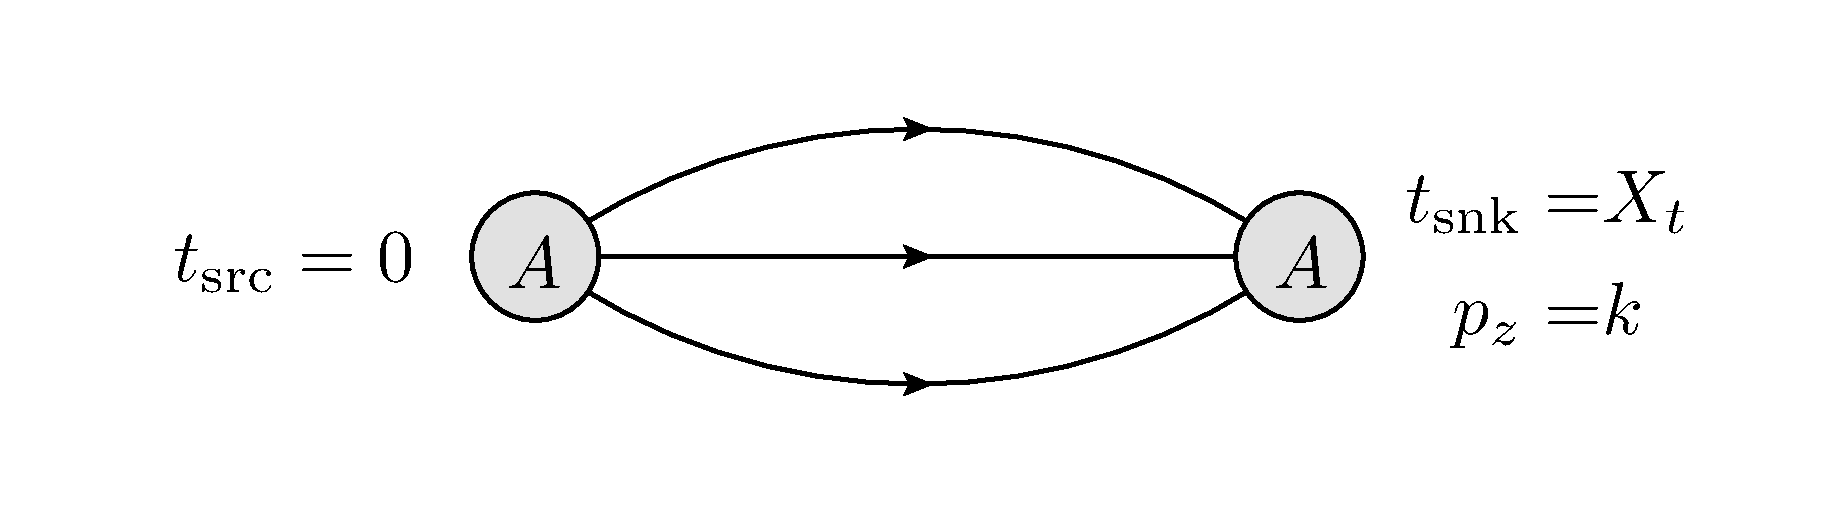
\includegraphics[width=0.75\textwidth]{./2pt_kinematics.pdf}
%	\caption{Kinematics of the two-point correlator with baryon initial and final states. We work in the rest frame of the final hadron. The diagram for semi-leptonic decays involves only one spectator quark, but involves the same kinematics.}
%	\label{fig:2pt_kinematics}
%\end{figure}

Given a two-point correlator with three-momentum $k$ in the $z$-direction,
\begin{align}
C_{\text{2pt}}(t) = \int d^3\vec{X} \left< A_{X_t,\vec{X}} | A_{0,\vec{0}}\right> e^{-ikX_z},
\label{eq:2pt}
\end{align}
where we use translation invariant to set the source at the origin, we can derive the derivative of the two-point correlator with respect to $k^2$,
\begin{align}
C^\prime_{\text{2pt}}(t) \equiv & \frac{\partial}{\partial k^2} C_{\text{2pt}}(t),  \nonumber\\
= & \int d^3\vec{X} \left<A_{X_t, \vec{X}} | A_{0,\vec{0}} \right> \left(\frac{-X_z}{2k}\right) \sin\left(kX_z\right),
\label{eq:2ptmoment}
\end{align}
where analogous to the moment of the three-point correlator, the cosine contribution vanishes due to symmetry.  Consequently, in the zero-momentum limit,
\begin{align}
\lim_{k^2\rightarrow 0 } C^\prime_{\text{2pt}} = \int d^3\vec{X} \left(\frac{-X_z^2}{2}\right)\left<A_{X_t, \vec{X}} | A_{0,\vec{0}} \right>.
\label{eq:2ptmoment0}
\end{align}
\dgr{\bfseries Again, similar comments apply both in terms of
  translation invariance and notation to the three-point function.}
The construction of the moment of the two-point correlator is similar
to the moment of the three-point correlator with the exception that
the moment now depends on the final state position $X_z$ instead of
the current insertion position $Y_z$. In both cases, the spatial
moments at all momenta are even, resulting in a non-vanishing
correlator under the Fourier transform, explicitly circumventing the
concern raised in Ref~\cite{Wilcox:2002zt}.  Given prior computational
investment in generating the
%two- and three-point correlators,
\dgr{propagators and sequential propagators, the}
generation of the moments of correlators only differ during the
Fourier transform, and therefore require negligible additional
computing time to construct.

\subsection{Interpretation}
\dgr{\bfseries This next sentence again may be a little pedantic for the audience, and would just remove it.  ``The time behaviour of the three-point correaltor of eqn 2.1 is given by'' and then use $C_{3pt}(t_x, t_y; k)$}
The space-time dependence of the correlator is made explicity by
moving to the Heisenberg representation. The fit ansatz to the
standard three-point correlator given by Eq.~(\ref{eq:3pt}) is,
\begin{align}
\left<A_{X_t,\vec{X}}|\Gamma_{Y_t,\vec{Y}}|B_{0,\vec{0}}\right> = & \sum_{n,m} \frac{\left<A | n\right>\left<n| \Gamma |m\right>\left<m | B\right>}{4E^A_n E^B_m} e^{-E^A_n(X_t - Y_t)} e^{-E^B_m Y_t} \label{eq:3ptfit},
\end{align}
where we Wick rotate to imaginary time, yielding a sum of \dgr{terms}
that decay exponentially in time.
%In the large $X_t$ and $Y_t$, limit,
\dgr{ In the limit of large $t_y$ and $t_x - t_y$,}
we recover the ground state contribution. \dgr{\bfseries This next sentence should be earlier.} The operators $A$ and $B$ are
interpolating operators, and have overlap with an infinite tower of
states labelled by $n$ and $m$ with corresponding eigenvalues $E_n$
and $E_m$ respectively.

Substituting Eq.~(\ref{eq:3ptfit}) into Eq.~(\ref{eq:3pt}), the
derivative of the three-point correlator follows,
\begin{align}
C^\prime_{\text{3pt}}(t_x, t_y) = & \frac{\partial}{\partial k^2} \int
d^3\vec{X} \int d^3\vec{Y} \sum_{n,m} \frac{\left<A | n\right>\left<n|
  \Gamma |m\right>\left<m | B\right>}{4E^A_n E^B_m} e^{-E^A_n(X_t -
  Y_t)} e^{-E^B_m Y_t} e^{-ikY_z}.
\end{align}
Performing the integral over $d^3\vec{X}$ projects the initial state
to zero momentum; the integral over $d^3 \vec{Y}$ projects momentum
$k$ to the current insertion while conservation of three-momentum
ensures that the final state also has three-momentum $k$. Therefore,
\begin{align}
C^\prime_{\text{3pt}}(t_x, t_y) = \frac{\partial}{\partial k^2}
\sum_{n,m} C_{nm}^{\text{3pt}} = \frac{\partial}{\partial k^2}
\sum_{n,m} \frac{Z_n^{\dagger A}(0) \Gamma_{nm}(k^2)Z_m^B(k^2)}{4
  M^A_n(0) E^B_m(k^2)} e^{-M^A_n(0)(X_t - Y_t)} e^{-E^B_m(k^2) Y_t},
\end{align}
where we define $Z_n^{\dagger A}(k^2) \equiv\left<A|n\right>$,
$\Gamma_{nm}(k^2) \equiv \left<n| \Gamma | m \right>$, $M_n^A(0)$ as
the rest mass of the $n$-th state of the interpolating operator $A$,
and \dgr{$E_n^B(k^2) = \sqrt{(M_n^B)^2+k^2}$} is the energy. Taking
the derivative with respect to $k^2$ yields,
\begin{align}
C^\prime_{\text{3pt}}(t_x, t_y) = &\sum_{n,m} C^{\text{3pt}}_{nm}\left\{ \frac{\Gamma_{nm}^\prime}{\Gamma_{nm}} + \frac{Z^{B\prime}_m}{Z^B_m} - \frac{1}{2(E_m^B)^2} -\frac{Y_t}{2E^B_m}\right\} \label{3ptmomentfit},
\end{align}
where $C_{nm}^{\text{3pt}}$ are the individual $n$ and $m$
contributions to the three-point correlator, and the prime denotes the
first derivative with respect to three-momentum $k^2$. The derivative
does not act on $Z^A$, which is in the rest frame of the initial
particle regardless of momentum transfer at the current. The
derivative only acts on $Z^B$ when \dgr{the operator B} is constructed from non-local
(smeared) interpolating operators, \dgr{since the smearing introduces an additional momentum
  scale}.
%, since a delta function source
%provides equal support to all eigenmodes.
\dgr{We are able to obtain $Z^{B\prime}_n$ by looking at the moment of
  the two-point correlator constructed frp, the operator $B$, as we now show.
We begin by using completeness to write the two-point correlator as}
\begin{align}
C_{\text{2pt}}(t) \equiv \left<B_{X_t,\vec{X}} | B_{0,\vec{0}}\right> = & \sum_m \frac{\left<B | m\right>\left<m | B\right>}{2E_m^B} e^{-E_m^B X_t} \label{eq:2ptfit}.
\end{align}
whence
%Substituting Eq.~(\ref{eq:2ptfit}) into Eq.~(\ref{eq:2pt}),
\begin{align}
C^\prime_{\text{2pt}}(t)=\frac{\partial}{\partial k^2} \int d^3\vec{X} \sum_m \frac{\left<B | m\right>\left<m | B\right>}{2E_m^B} e^{-E_m^B X_t} e^{-ikX_z},\label{eq:2ptprime}
\end{align}
The integral over $X_z$ projects the state to
\dgr{definite momentum $k$}.
%to the
%sink injects momentum $k$ to the source through three-momentum
%conservation.
%The moment of the two-point correlator is modeled by the
%following fit ansatz,
\dgr{Applying the $k^2$ derivative to the right-hand-side of
Eq.~(\ref{eq:2ptprime}) yields}
\begin{align}
C^\prime_{\text{2pt}} =\frac{\partial}{\partial k^2} \sum_m C_m^{\text{2pt}}= & \frac{\partial}{\partial k^2} \sum_m \frac{Z^{B\dagger}_m(k^2)Z^B_m(k^2)}{2E^B_m(k^2)}e^{-E_m^B(k^2)X_t},\\
= & \sum_m C^{\text{2pt}}_m \left(\frac{2Z_m^{B\prime}}{Z_m^B} - \frac{1}{2[E_m^B(k^2)]^2}-\frac{X_t}{2E_m^B(k^2)}\right).
\end{align}

%\dgr{Observables such as the charge radius are defined through the derivative
with respect to the
four-momenta, $q^\mu \equiv (E_m^B(k) - M_n^A,0,0,k), Q^2 = - q^2$, where for a fixed
three three-momentum $k$ the four momentum depends on the energies of
the ingoing and outgoing states.
%momenta now depends on the ingoing and outgoing states in the
%two-point and three-point correlations.
The connection between the three- and four-momentum derivatives arises
from the chain rule,
\begin{align}
\frac{\partial}{\partial k^2} \Gamma_{nm} = & \frac{\partial Q^2}{\partial k^2}\frac{\partial}{\partial Q^2}\Gamma_{nm},\\
= & \frac{M^A_n}{\sqrt{(M^B_m)^2+k^2}}\frac{\partial}{\partial Q^2} \Gamma_{nm}.
\end{align}
\dgr{\bfseries I don't think we need necessarily to describe this any
  further, at least for the lattice writeup}.
%where $q^\mu$ is the 4-momentum of the current insertion. Four-momentum conservation requires the momentum at the current insertion be,
%\begin{align}
%q^\mu = & \begin{pmatrix} \sqrt{\left(M_m^B\right)^2+k^2}-M_n^A & 0 & 0 & k\end{pmatrix},\\
%\therefore -Q^2\equiv q^2 = & \Delta^2_{mn} + 2M^A_n \left( M^A_n-\sqrt{\left(M^B_m\right)^2+k^2}\right),
%\end{align}
%where $\Delta_{mn} \equiv (M^B_m)^2 - (M^A_n)^2$.

\section{Charge radius of the proton}
We demonstrate our method by calculating the charge radius of the
proton on the 2+1 flavor William and Mary / JLab isotropic clover
ensemble.  We use the ensemble with lattice spacing $a \simeq
0.12~{\rm fm}$, with a box size of $N_s^3\times N_t = 24^3\times 64$
with a pion mass of 400~MeV. To minimize the dominant error, which is
the finite volume effects experience by the valence quarks, we work on
a lattice replicated in the $z$-direction to yield a $N_{x,y}^2 \times
N_z \times N_t = 24^2\times 48\times 64$ lattice.  A total of 480
configurations with 16 sources are analyzed in the follow results.

\subsection{Spatial propagation of the correlator}
Lattice calculations are performed in Euclidean space-time, leading to
only space-like separations.  Therefore, propagation in all space-time
directions are exponentially damped. We show that the two- and
three-point correlators used to calculate the charge radius exhibit
this behavior in the spatial direction. As a result, the correlators
are local, and the integral of the correlators with any polynomial
moment in space converge, yielding exponentially suppressed finite
volume effects.

\begin{figure}[h]
	\centering
		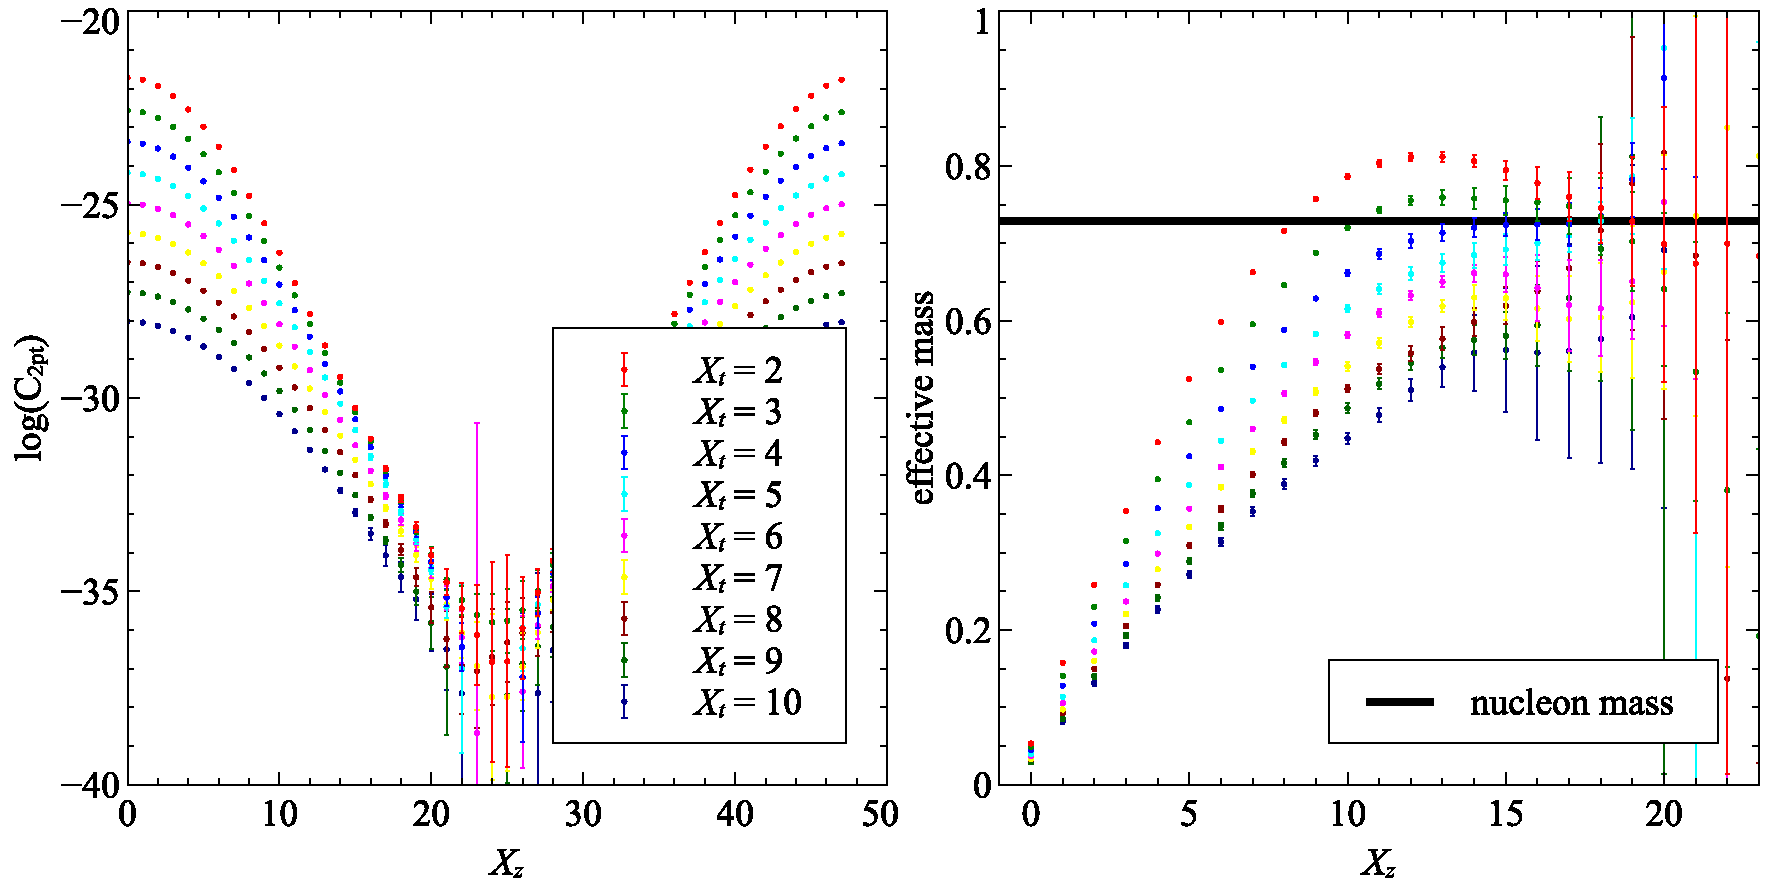
\includegraphics[width=0.85\textwidth]{./2ptzcorr.pdf}
	\caption{(Left) The log of the two-point correlator as a function of spatial separation at fixed time separations. At large spatial separations, the correlator behaves linearly.  (Right) The effective mass of the correlator is plotted as a function of spatial separation at fixed time slices.  A plateau is observed around the nucleon mass. The black band marks the nucleon mass obtained from a fit to the two-point correlator.}
	\label{fig:2pt_zcorr}
\end{figure}

In Fig.~\ref{fig:2pt_zcorr}, we show the log of the two-point correlator as a function of spatial separation for the array of time separations used in the correlator analysis presented later. We observe that at large spatial separations, the correlator is linear, suggesting exponential damping. The corresponding effective mass plot shows saturation at large spatial separations around the nucleon mass, where the black band labels the nucleon mass determined from a fit to the two-point correlator.

\begin{figure}[h]
	\centering
		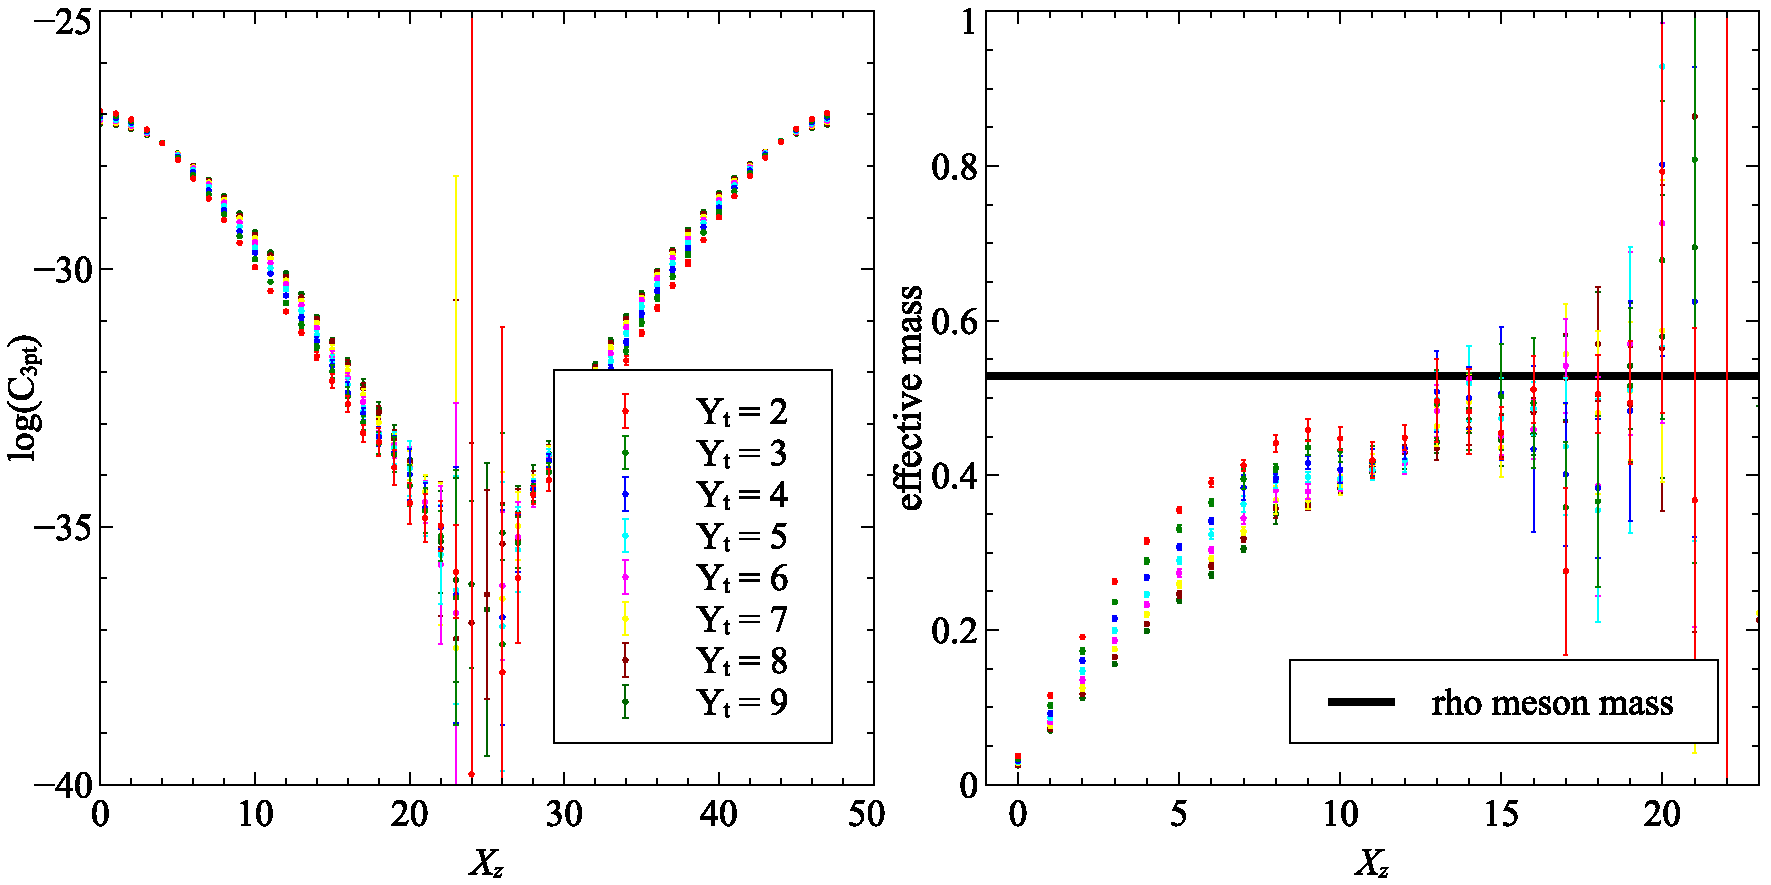
\includegraphics[width=0.85\textwidth]{./3ptzcorr.pdf}
	\caption{Analogous to Fig~\ref{fig:2pt_zcorr}, the log of the three-point correlator, and the corresponding effective mass is presented. In the case of the three-point, we observe exponential damping mediated by the rho meson mass.}
	\label{fig:3pt_zcorr}
\end{figure}

The spatial propagation of the three-point correlator is analogous to the two-point correlator.  In our example however, the lowest lying state in the three-point corresponds to the vector meson created by the current insertion. We analytically integrate the spatial dimensions of the three-point to eludicate the exponential damping observed. We construct space-like Feynman propagators in the spatial direction by position-ordering the operators and make explicit the space-time dependence by moving to the Heisenburg representation,
\begin{align}
C_{\text{3pt}}^\prime(X,Y) = &2\sum_{n,m}\int_{0}^{\infty}d\vec{X}d\vec{Y} M(Y_z)\frac{Z_n^{A\dagger}\Gamma_{nm}Z_m^B}{4E_n^AE_m^B}e^{-E_n^AX_z}e^{-(E_m^B-E_n^A)Y_z}F^{\text{in}}(X_t,Y_t)\Theta(X_t-Y_t)\nonumber\\
&+2\sum_{n,r}\int_{0}^{\infty}d\vec{X}d\vec{Y}M(Y_z) \frac{\Gamma_{r}Z_{rn}^{A\dagger}Z_n^B}{4E_r^\Gamma E_n^B}e^{-E_r^\Gamma Y_z}e^{-(E_n^B-E_r^\Gamma)X_z}F^{\text{out}}(X_t,Y_t)\Theta(Y_t-X_t),
\end{align}
where the first term describes the the current insertion between the two hadrons, while the second term has the current insertion outside. The symmetric moment for arbitrary momenta is defined as $M(Y_z)\equiv\frac{-Y_z}{2k}\sin{(kY_z)}$. The functions $F^{\text{in},\text{out}}$ parameterizes the standard time dependence of a three-point correlator that are irrelevant to this discussion, but are detailed in Eq.~(\ref{eq:3ptfit}). The correlator exponentially and symmetrically damps away from the origin, allowing us to integrate twice over the positive axis.	 Collecting the QCD matrix elements and time dependence into $G_{nm}$ and $H_{nr}$, we first integrate over the sink before integrating over the current insertion,
\begin{align}
C^\prime_{\text{3pt}}(X,Y) = &2\sum_{n,m}G_{nm}\int_0^\infty dY_z M(Y_z)e^{-(E_m^B-E_n^A)Y_z}\int_{Y_z}^\infty dX_z e^{-E_n^A X_z}\nonumber\\
&+2\sum_{n,r}H_{nr}\int_0^\infty dY_z M(Y_z)e^{-E_r^\Gamma Y_z}\int_0^{Y_z}dX_z e^{-(E_n^B-E_r^\Gamma)X_z},\nonumber\\
=&\sum_{n,m}\frac{2G_{nm}}{E_n^A}\int_0^\infty dY_z  M(Y_z)e^{-E_m^B Y_z} - \sum_{n,r}\frac{2H_{nr}}{E_n^A-E_r^\Gamma}\int_0^\infty dY_z  M(Y_z) \left(e^{-E_n^B Y_z}-e^{-E_r^\Gamma Y_z}\right),
\end{align}
and conclude that the spatial integral converges in the infinite volume limit. The lowest-lying state is operator dependent, but for the charge radius, $E_0^\Gamma$ corresponds to a rho-like meson at rest, and is lighter than $E_0^B$ the rest mass of the nucleon as demonstrated by Fig.~\ref{fig:3pt_zcorr}.

\subsection{Correlator analysis}
We perform a Bayesian constrained curve fit simultaneously to the two-point correlator, three-point correlators, and their respective moments. For the three-point correlator, we include two sink locations to disentangle excited state contributions. However, we only work with Gaussian smeared source and sink operators to suppress these excited states. Finally, we only work with the connected contribution to the vector form factor of the proton.

The ground state priors are motivated from looking at the standard effective mass and scaled correlator plots. The width of these ground state priors are orders of magnitude wider compared to the posterior distribution, rendering them effectively unconstrained. The excited state energies are defined as a tower of splittings with lognormal distributions where the mean is $2m_\pi$ and the width is of the same order of magnitude. Priors for the excited state overlap factors, matrix elements, and slopes are chosen to have a mean of zero, with a width that is five times the ground state central value.

\begin{figure}[h]
	\centering
		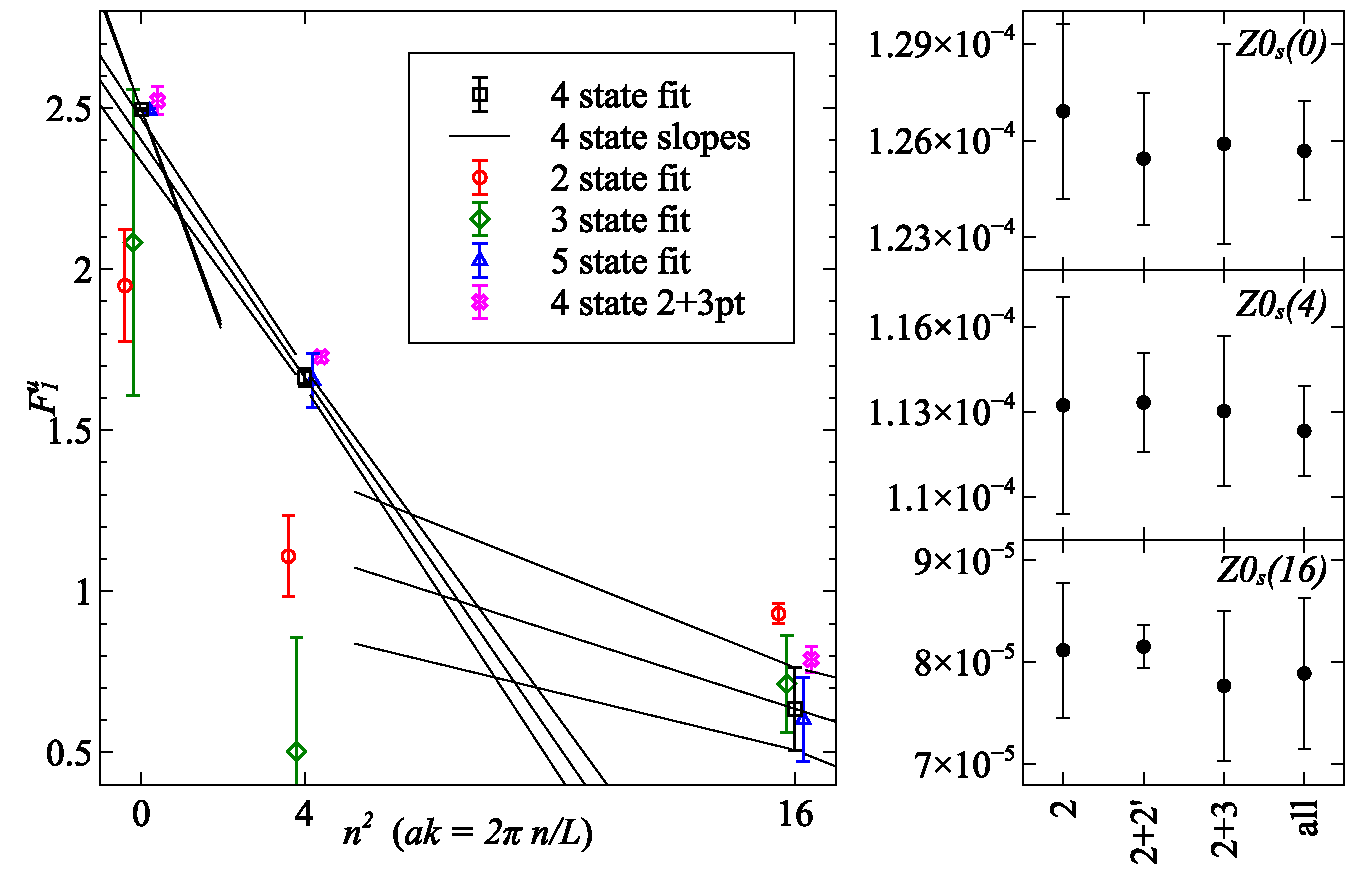
\includegraphics[width=0.9\textwidth]{./gV.pdf}
	\caption{{\color{red} This caption is wayyyy too long :(}(Left) Fit of $F_1^u$, the connected contribution to the proton axial form factor. For all relevant fits, the two-point correlator fit region spans time separations of 2 to 10, the moment of the two-point correlator spans time separations of 3 to 11. The three-point correlator with $T_{\text{snk}}=10$ is fit with current insertion times of 2 to 8, while $T_{\text{snk}}=12$ has time separations spanning 2 to 10; the corresponding three-point moments fit regions span 4 to 8 and 4 to 9 for the two sink separations respectively. For the preferred fit with 4 states in the fit ansatz, the $\chi^2_\text{aug}/\text{d.o.f.}$ is 2.0, with the data contributing to 80\% of the total $\chi^2$; the augmented-$\chi^2$ is the sum of the $\chi^2$ contribution from data and the $\chi^2$ contribution from priors~\cite{Lepage:2001ym}. (Right) We check stability under fitting over subsets of data, for simultaneous fits of 2: exclusive two-point, $2+2^\prime$:two-point plus two-point moment, 2+3: two-point with three-point, all: two-point, two-point moment, three-point, and three-moment.}
	\label{fig:gV}
\end{figure}

We demonstrate full control over fit systematics by checking for stability under varying fit region, ground state prior widths and number of states included in the fit ansatz. In Fig.~\ref{fig:gV}, we plot our result for the vector form factor $F^u_1$ at three different lattice momenta, and show control of excited state systematics.  The preferred fit is marked by the black square, with corresponding slopes extracted from the simultaneous correlator fit. We vary the number of states in our fit ansatz from 2 (red circle), 3 (green diamond), and 5 (blue triangle), and observe that including and beyond 4 states, the central values of $F_1^u$ stabilize. We further compare the value of $F_1^u$ against a simultaneous two- and three-point fit (pink cross), and observe consistency. The three panels on the right side of Fig.~\ref{fig:gV} compare the ground state overlap factors obtained from a two-point correlator, two-point correlator with its moment, two- and three-point correlator, and finally the full simultaneous fit to all correlators.  The consistency of the ground state overlap factors between different subsets of data futher demonstrate confidence in our fit analysis. We observe promising results from this method; the slopes for the three-values of lattice momenta agree well with expectation, and the uncertainty of the slopes are of the same order, but slightly larger, than the uncertainty on $F_1^u$.

\section{Outlook}
In these proceedings, we present a method to calculate slopes at arbitrary lattice momenta for matrix elements directly on the lattice.  Immediately interesting applications include calculating the isovector axial radius to obtain $F_A(q^2)$ and the charge radius of the proton.  In particle physics, this method may help further constrain CKM phenomenology through stronger constraints on the shape of weak decay form factors. The proposed method is computationally cheap to implement and therefore is suitable to implement as an exploratory study in a wide range of physics applications.

\bibliographystyle{physrev} %%% physical review
\bibliography{PCR} %%% bib file

\end{document}
